\documentclass[11pt,a4paper]{article}
\usepackage{amsmath}
\usepackage{amssymb}
\usepackage{graphicx}
\usepackage{verbatim}
\begin{document}
\noindent
Martin Lundfall, Henri Bunting, Malte Siemers, Patrik Bey
\begin{centering}
  \section*{Exercise sheet 10 - Machine Intelligence I}
  \end{centering}
  
    \subsection*{10.1 - Directed Acylic Graphs and Graphical Models}
  
  \subsubsection*{(a)} Nodes represent the random variables, edges the correlative relationship between those nodes, and the edge direction symbolizes causation.
  \subsubsection*{(b)} Two nodes are conditionally independent if their combined probability, given a parent, is equal to the product of individual probabilities of the nodes given the parent.  This enables a decomposition of the graph.  Conditional Independence is shown in the graph structure as a lack of edges between nodes. 
  \newpage
  \subsubsection*{(c)} 
  Here is a step-by-step visualization of the algorithm.\\
  \begin{figure*}[h]
  	\begin{minipage}[t]{4 cm}
		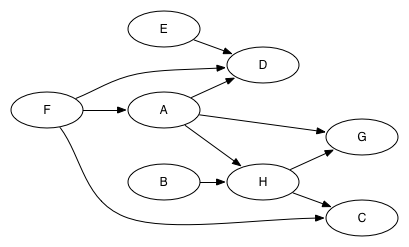
\includegraphics[width=\linewidth]{101c0}
		\caption{initial state}
  	\end{minipage}
  	\begin{minipage}[t]{4 cm}
		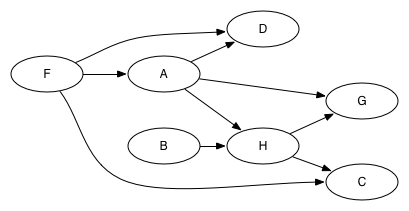
\includegraphics[width=\linewidth]{101c1}
		\caption{i = 1}
  	\end{minipage}
  	\begin{minipage}[t]{4 cm}
		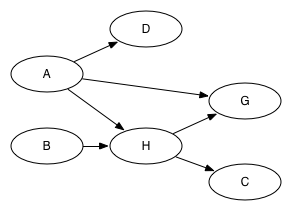
\includegraphics[width=\linewidth]{101c2}
		\caption{i = 2}
  	\end{minipage}
  	\begin{minipage}[t]{4 cm}
		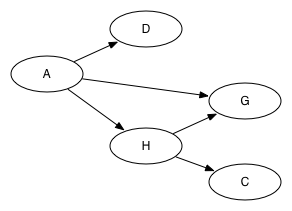
\includegraphics[width=\linewidth]{101c3}
		\caption{i = 3}
  	\end{minipage}
  	\begin{minipage}[t]{4 cm}
		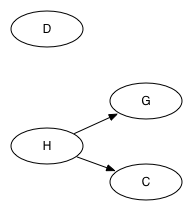
\includegraphics[width=\linewidth]{101c4}
		\caption{i = 4}
  	\end{minipage}
  	\begin{minipage}[t]{4 cm}
		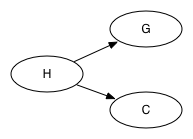
\includegraphics[width=\linewidth]{101c5}
		\caption{i = 5}
  	\end{minipage}
  	\begin{minipage}[t]{4 cm}
		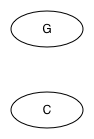
\includegraphics[width=\linewidth]{101c6}
		\caption{i = 6}
  	\end{minipage}
  	\begin{minipage}[t]{4 cm}
		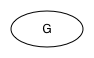
\includegraphics[width=\linewidth]{101c7}
		\caption{i = 7}
  	\end{minipage}
  \end{figure*}\\
  This results in the topological sorting: E,F,B,A,D,H,C,G
  \newpage
  \subsubsection*{(d)} The factorization of join distribution for the DAG is:\\
  $P(F) * P(E) * P(B) * P(A|F) * P(D|E,A,F) * P(H|B,A,F) * P(G|H,B,A,F) * P(C|H,B,A,F)$\\
  Given conditional independence, this can be reduced to:\\
  $P(F) * P(E) * P(B) * P(A|F) * P(D|E,A) * P(H|B,A) * P(G|H,A) * P(C|H,F)$
  \subsubsection*{(e)} The Markov Blanket of the node, A, is: $\{F,B,E,D,H\}$\\
  Where:\\
  $\{F\}$ is the parent node\\
  $\{D,H\}$ are children nodes\\
  $\{B,E\}$ are the children's parents nodes
  \subsubsection*{(f)} A naive Bayes Classifier assigns a class label to a node $x$ based on the class's probability and the probability of the node belonging to that class.\\
  \begin{equation}
  	\bar{y} = \underset{k}{\text{argmax}} P(C_{k})\prod_{i}P(x_{i}|C_{k})
  \end{equation}
  
  
\subsection*{10.3}
\subsubsection*{a)}
Representing the probabilities as a DAG, we see the following dependencies:
\begin{figure}[h]
  \centering
  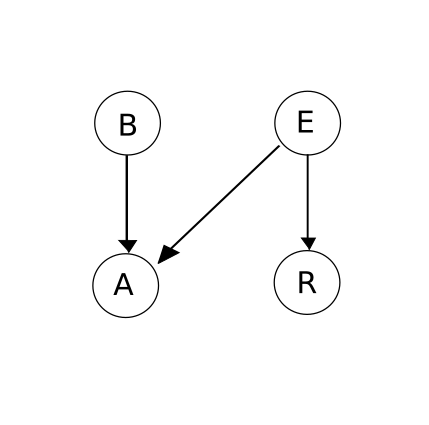
\includegraphics[width=.4\textwidth]{graph}
    \caption{DAG illustrating probability dependencies}
  \end{figure}
\subsubsection*{b)}
Explaining away descibes the phenomenon of independant random variables getting dependant in the case where both of them are the condition for a shared event. If this event is obsereved, both of the conditions are 'competing' to have caused it. A prior knowledge of one of the causing variables will then have a certain effect on the other. To illustrate this concept, in our examplary DAG we consider the case where the alarm has gone off while there was a radio broadcast. What are the respective probabilities of a burglary having occured?\\
The probability of a burglary not having occured is:
\begin{equation*}
  \begin{split}
  P(B=f|A=t,E=t)  = \frac{P(E=t, A=t | B=f)P(B=f)}{P(A=t,E=t)}=\\
  \\
  =  \frac{P(A=t |E=t, B=f)P(B=f)P(E=t)}{P(A=t|E=t)P(E=t)}= \\
  \\
  =  \frac{P(A=t| B=f, E=t)P(B=f)}{P(A=t|B=t,E=t)P(B=t)+P(A=t|B=f,E=t)P(B=f)} = \\
  = \frac{0.41*0.99}{0.98*0.01+0.41*0.99}=0.97642...
  \end{split}
\end{equation*}
The probability of a burglary having occured is:
\begin{equation*}
  \begin{split}
  P(B=t|A=t,E=t)  = \frac{P(E=t, A=t | B=t)P(B=t)}{P(A=t,E=t)}= \\
  \\
  =  \frac{P(A=t |E=t, B=t)P(B=t)P(E=t)}{P(A=t|E=t)P(E=t)}= \\
  \\
  =  \frac{P(A=t| B=t, E=t)P(B=t)}{P(A=t|B=t,E=t)P(B=t)+P(A=t|B=f,E=t)P(B=f)} \\
  = \frac{0.98*0.01}{0.98*0.01+0.41*0.99}=0.02357...
  \end{split}
\end{equation*}
We see that if there was a radio broadcast while the alarm went off, a burglary probably hasn't occured. This seems to indicate that keeping the radio on reduces the risk for burglaries, but this is a faulty assumtion to make, since the two probabilities are independent.\\
An other exsample would be the occurence of a warm or a cold day. In spring there might be a 0.5 chance for both of them. On the cold day I might turn on my heater with a higher chance than on a hot day and I might leave the window open on a hot day (that will render the insides of my room warm) with a higher chance than on a cold one. In the end, my room will might be observed as warm. If I now know I left the window open, the chances of me having the heater turned on are small. 
\end{document}
